\documentclass[twoside, 11pt]{article}
\usepackage{amsmath}
\usepackage{amssymb}
\usepackage[colorlinks=true, citecolor=blue, linkcolor=black]{hyperref}
\usepackage{listings}
\usepackage{xcolor}
\usepackage{graphicx}

%\usepackage[sc]{mathpazo} % Use the Palatino font
\usepackage[T1]{fontenc} % Use 8-bit encoding that has 256 glyphs
\linespread{1} % Line spacing - Palatino needs more space between lines
\usepackage{microtype} % Slightly tweak font spacing for aesthetics

\usepackage[hmarginratio=1:1,top=32mm,columnsep=20pt]{geometry} % Document margins
\usepackage{multicol} % Used for the two-column layout of the document
\renewcommand{\figurename}{\bfseries\scshape Fig.}
\renewcommand{\tablename}{\bfseries\scshape Table}
\usepackage[hang, small,labelfont=sc,up,textfont=normalfont,up]{caption} % Custom captions under/above floats in tables or figures
\usepackage{float} % Required for tables and figures in the multi-column environment - they need to be placed in specific locations with the [H] (e.g. \begin{table}[H])
\usepackage{hyperref} % For hyperlinks in the PDF

\usepackage{listings}
\lstset{language=C++,
				backgroundcolor=\color{black!5},
                basicstyle=\scriptsize ,
                keywordstyle=\color{blue}\ttfamily,
                stringstyle=\color{red}\ttfamily,
                commentstyle=\color{green}\ttfamily,
                morecomment=[l][\color{magenta}]{\#},
                tabsize = 1,
}

\usepackage{abstract} % Allows abstract customization
\renewcommand{\abstractnamefont}{\normalfont\bfseries} % Set the "Abstract" text to bold
\renewcommand{\abstracttextfont}{\normalfont\small\itshape} % Set the abstract itself to small italic text

\usepackage{titlesec} % Allows customization of titles
%\renewcommand\thesection{\textbf{\Roman{section}}} % Roman numerals for the sections
%\renewcommand\thesubsection{\roman{subsection}} % Roman numerals for subsections
\titleformat{\section}[block]{\bf\Large\scshape\centering}{\thesection.}{1em}{} % Change the look of the section titles
\titleformat{\subsection}[block]{\bf\large\scshape\centering}{\thesubsection}{1em}{} % Change the look of the section titles
\titleformat{\subsubsection}[block]{\bf\normalsize\scshape\centering}{\thesubsubsection}{1em}{}

\usepackage{fancyhdr} % Headers and footers
\pagestyle{fancy} % All pages have headers and footers
\fancyhead{} % Blank out the default header
\fancyfoot{} % Blank out the default footer
\fancyhead[C]{FYS3150 - Computational physics $~ \cdot ~$ Project 3} % Custom header text
\fancyfoot[C]{\small\thepage} % Custom footer text

%----------------------------------------------------------------------------------------
%	TITLE SECTION
%----------------------------------------------------------------------------------------

\title{\vspace{-15mm}\fontsize{16pt}{13pt}\selectfont\textbf{Numerical integration using Gaussian quadrature- and Monte Carlo methods}} % Article title

\author{
\large
Ole Gunnar Johansen\\[0mm]%\thanks{A thank you or further information}\\[2mm] % Your name
\normalsize University of Oslo \\[0mm] % Your institution
\normalsize \href{mailto:olegjo@ulrik.uio.no}{olegjo@student.matnat.uio.no} % Your email address
\vspace{5mm}
}
\date{}

\renewcommand{\d}{\mathrm{d}}

\begin{document}
\maketitle % Insert title
\thispagestyle{fancy} % All pages have headers and footers


\begin{abstract}

\noindent
In this project, I have been looking at the infinite six-dimensional integral needed to find the expectation value of the quantum mechanical correlation energy between two electrons in the helium atom. I have been using Gauss-Legendre quadrature, Gauss-Laguerre quadrature, a "brute force" Monte Carlo approach, and finally a Monte Carlo approach with importance sampling. Computation times are compared for all methods and the latter method produced very good results in a matter of a few seconds, and the first did not produce comparable results even after 7 minutes. 
\end{abstract}

%\begin{multicols}{1}

\section{Introduction}
	Integrals play a huge role in science. Many of the integrals we encounter are possible to evaluate analytically, but a vast sample is not and numerical methods have to be used. Numerical integration is, however, prone to round off errors, especially if the functions which we are evaluating do not behave "nicely". The Newton-Cotes algorithm is a very easy algorithm to implement and understand, however it doesn't produce very reliable results. Supplementing this algorithm, there have been developed a lot of other schemes. In this project, I have implemented Gaussian quadrature with weight functions based on Legendre polynomials and Laguerre polynomials, as well as two Monte Carlo methods to solve a quantum mechanical integral, specifically the quantum mechanical expectation value of the correlation energy between two electrons which repel each other via the classical Coulomb interaction. 
	
	The integral in question can be solved in closed form and its exact value is therefore used in the discussion of the reliability of the different methods.

\section{Theory/Methods}
	\subsection{The Integral}
		The integral we will evaluate is the six-dimensional ground state expectation value of the correlation energy between to electrons in a helium atom. To do this, we assume that each electron can be modelled via the single-particle wave function
		\begin{align}
			\psi_{1s} (\mathbf{r}_i) = e^{-\alpha r_i}
		\end{align}
		where $\alpha$ is a parameter corresponding to the charge of the nucleus around which the electrons are orbiting, the position vector $\mathbf{r}_i$ for electron $i$ is given by
		\begin{align}
			\mathbf{r}_i = x_i \mathbf{e}_x + y_i \mathbf{e}_y + z_i \mathbf{e}_z
		\end{align}
		with magnitude
		\begin{align}
			r_i = \sqrt{x_i^2 + y_i^2 + z_i^2}.
		\end{align}
		
		The wave function for two electrons is then given by
		\begin{align}
			\Psi(\mathbf{r}_1, \mathbf{r}_2) = \psi(\mathbf{r}_2)\psi(\mathbf{r}_2) = e^{-\alpha(r_1 + r_2)}
		\end{align}
		Note that this is not normalized, however this will only change the integral by a factor equal to the normalization factor, and is not of interest in this project.
		
		The integral which we wish to solve is then
		\begin{align}
			\langle \frac{1}{|\mathbf{r}_1 - \mathbf{r}_2|} \rangle = \int_{-\infty}^{\infty} \d\mathbf{r}_1 \mathbf{r}_2 e^{-2\alpha(r_1+r_2)} \frac{1}{|\mathbf{r}_1 - \mathbf{r}_2|} \label{eq: unchanged integral}
		\end{align}
		where the differentials $\mathbf{r}_i$ are the volume elements in Cartesian coordinates. The above integral has the closed form answer $5\pi^2/16^2$.
		
		Numerically, the integration limits of $\pm \infty$ are difficult to implement. However, if we make a change of variables to spherical coordinates, we loose 4 out of six infinite integrals.
		In spherical coordinates, the volume elements can be written as
		\begin{align}
			\d\mathbf{r}_i = r_i^2\sin (\theta_i)\d \theta_i \d \phi_i \d r_i
		\end{align}
		where $r_i \in [0, \infty)$, $\theta_i \in [0, \pi]$ and $\phi_i \in [0, 2\pi]$. The magnitude of the distance between the electrons is 
		\begin{align}
			|\mathbf{r}_1 - \mathbf{r}_2| = r_{12} = \sqrt{r_1^2 + r_2^2 - 2r_1 r_2 \cos \beta}
		\end{align}
		where
		\begin{align}
			\cos\beta = \cos(\theta_1) \cos (\theta_2) + \sin(\theta_1)\sin(\theta_2) \cos(\phi_1 - \phi_2) \nonumber
		\end{align}
		The integral in spherical coordinates is then
		\begin{align}
			\langle \frac{1}{r_{12}} \rangle = \int \d r_1 \d r_2 \d \theta_1 \d \theta_2 \d \phi_1 \d \phi_2 \frac{1}{r_{12}} r_1^2r_2^2\sin(\theta_1)\sin(\theta_2) e^{-2\alpha(r_1+r_2)}
		\end{align}
		
		Simplifying further, using $u = 2\alpha r_1$ and $v = 2\alpha r_2$ ($u\in [0,\infty$, $v\in [0, \infty)$), we obtain finally
		\begin{align}
			\langle \frac{1}{r_{12}} \rangle = \frac{1}{(2\alpha)^5} \int \d u \d v \d \theta_1 \d \theta_2 \d \phi_1 \d \phi_2 \frac{1}{\sqrt{u^2 + v^2 - 2uv\cos\beta}} u^2v^2\sin(\theta_1)\sin(\theta_2) e^{-u}e^{-v} \label{eq: integral in spherical coordinates, u, v}
		\end{align}
		
	\subsection{Gaussian Quadrature}
		The basic idea behind Gaussian quadrature is to approximate the integral of a function $f$ by
		\begin{align}
			I = \int_{a}^{b} f(x) \ \d x  = \int_{a}^{b} W(x)g(x) \ \d x \approx \sum_{i=1}^N w_i g(x_i) \label{eq: gaussian quadrature basic idea}
		\end{align}
		where $W(x)$ is a weight function obtained through a polynomial which is orthogonal in some interval $[a, b]$. Two such weight functions are $W(x)=1$ which uses Legendre polynomials in the interval $x\in[-1, 1]$ and $W(x) = x^\alpha e^{-x}$ which uses the Laguerre polynomials in the interval $x \in [0, \infty)$. 
		
		\subsubsection{The 6-Dimensional Integral}\label{section: the 6-dimensional integral}
			Eq.~\eqref{eq: gaussian quadrature basic idea} shows the formalism for calculating a one-dimensional integral. For a multidimensional integral, it is quite similar, only we need a number of sums equal to the number of dimensions. In a computer program, this is done with $n$ for loops when $n$ is the number of dimensions. For the 6-dimensional case a code snippet could look like
			
			\begin{lstlisting}
double integral = 0;
for (int i=0; i < order; i++) {
		for (int j=0; j < order; j++) {
		for (int k=0; k < order; k++) {
		for (int l=0; l < order; l++) {
		for (int m=0; m < order; m++) {
		for (int n=0; n < order; n++) {
			integral += w_d1[i]*w_d2[j]*w_d3[k]*w_d4[l]*w_d5[m]*w_d6[n]*
						integrand(x_d1[i], x_2[j], x_d3[k], x_d4[l], x_d5[m], x_d6[n]);
		}}}}}
}
			\end{lstlisting}
			where \texttt{w\_di} and \texttt{z\_di} are arrays containing the weights and roots associated with the \texttt{i}-th dimension in the proper interval, and \texttt{integrand} is a function evaluating the integrand for the six dimensions. 
			
		
		\subsubsection{Gauss-Legendre Quadrature}
			As indicated above, the weight function used in Gauss-Legendre Quadrature is $W(x)=1$. The function which we wish to integrate is therefore the same, that is
			\begin{align}
				I = \int_{-1}^{1} f(x) \ \d x \approx \sum_{i=1}^N w_i f(x_i)
			\end{align}
			where $x_i$ are the abscissas  given by the roots of the Legendre polynomial $P_N$ of degree $N$ and $w_i$ are the weights given by
			\begin{align*}
				w_i = \frac{2}{(1-x_i^2)[P'_N(x_i)]^2}
			\end{align*}
			
			For this project, I have developed a code which returns the weights and  abscissas for the Legendre polynomial of degree $N$. The codes can be found in the file \texttt{gaussianquadrature.cpp}. The relevant functions are \texttt{legendreRoots} and \texttt{legendreWeights}.
			
			The function \texttt{legendreRoots} begins with an initial guess for the $i$-th root 
			\begin{align*}
				x_\mathrm{guess} = \cos \left( \pi \frac{4(i+1) - 1}{4N + 2} \right) 
			\end{align*}
			and then approximates the real root using Newtons method. 
			
			
			Note that the direct use of this method will integrate a function in the interval $x\in[-1,1]$. Our function is, however, in the limits $\pm \infty$. We can always change variables from the limits $x \in [a, b]$ to $x \in [-1, 1]$ using
			\begin{align}
				\int_{a}^{b} f(x) \ \d x = \frac{b-a}{2} \int_{-1}^{1} f\left( \frac{b-a}{2}x_i + \frac{b+a}{2} \right) \ \d x
			\end{align}
			which does not help us evaluating the infinite integrals of eq.~\eqref{eq: unchanged integral}. To deal with this problem, note that eq.~\eqref{eq: unchanged integral} involves an exponential on the form $e^{-x}$ which approached 0 quickly. To evaluate the integral using Gauss-Legendre quadrature, the limits $a$ and $b$ are therefore set to a value where $e^{-2\alpha r}$ is more or less zero. Fig.~\ref{fig: integration limits Gauss-Legendre} shows a plot of $e^{-\alpha |x|}$, and by inspection such limits could be set to $\pm 5$. 
			
			Since we are now working in Cartesian coordinates, all directions are weighted the same and we need only make one call to the functions that calculate the roots and weights of the Legendre polynomial, i.e. \texttt{w\_d1}=\texttt{w\_d2}=...=\texttt{w\_d6}=\texttt{w} and similarly  \texttt{x\_d1}=\texttt{x\_d2}=...=\texttt{x\_d6}=\texttt{x} in the code in section~\ref{section: the 6-dimensional integral}. The \texttt{integrand} function is now simply the integrand in eq.~\eqref{eq: unchanged integral}.
			
			\begin{figure}
				\centering
				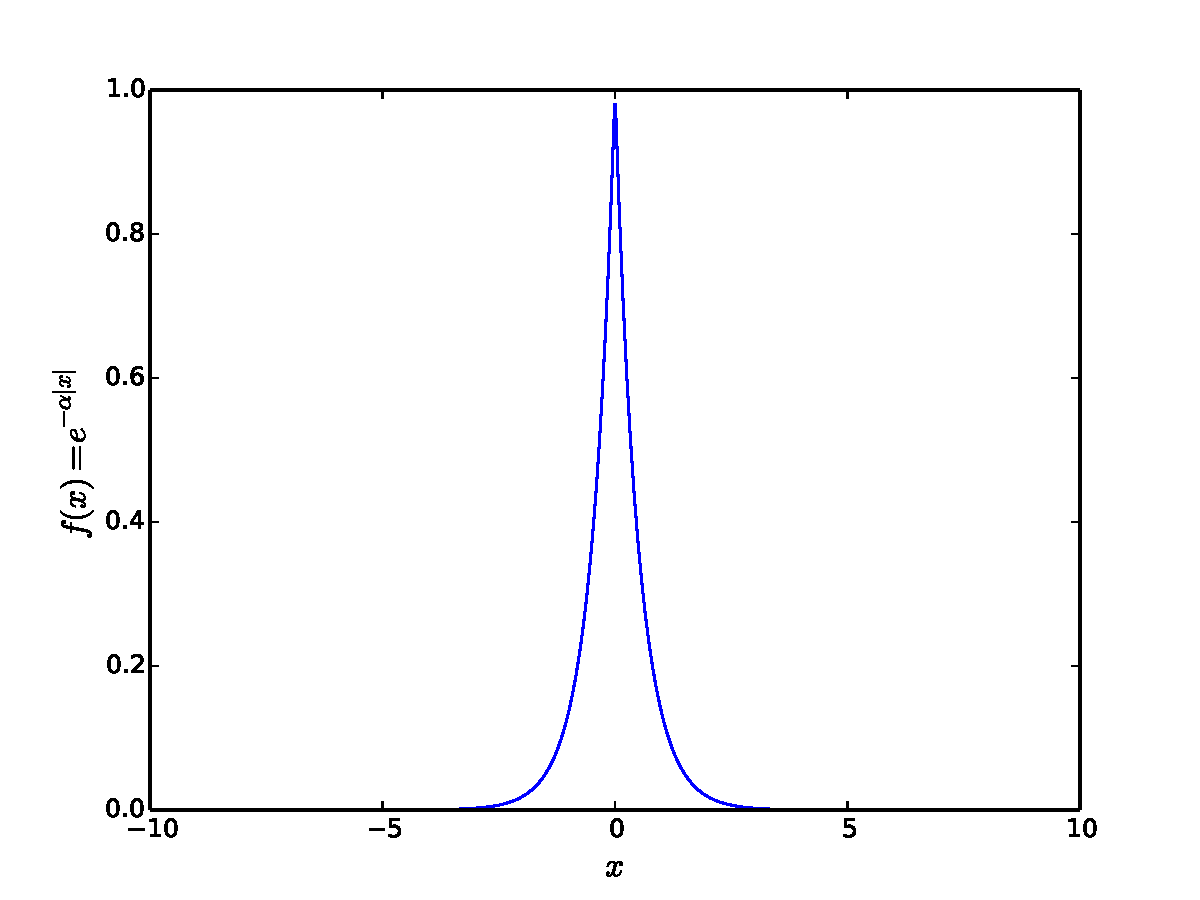
\includegraphics[scale=0.7, clip=true, trim= 0 0 0 0]{FYS3150-project-3-plot-taska-limits.pdf}
				\caption{Plot of $e^{-\alpha |x|}$ to find appropriate integration limits for Gauss-Legendre quadrature. We see that the function is more or less zero for $x\approx 5$.}
				\label{fig: integration limits Gauss-Legendre}
			\end{figure}
		
		
		\subsubsection{Gauss-Laguerre Quadrature}
			Gauss-Laguerre quadrature is somewhat more sophisticated than Gauss-Legendre. In this case, the weight function is given by $x^\alpha e^{-x}$ and the associated polynomial is the Laguerre polynomials which are orthogonal in the interval $x\in [0, \infty)$. Looking back at eq.~\eqref{eq: integral in spherical coordinates, u, v}, we see that this rewriting of the original integral involves factors of the kind $x^\alpha e^{-x}$, and so, using the formalism in eq.~\eqref{eq: gaussian quadrature basic idea}, these factors can be taken out of the integral when we are employing a proper polynomial, namely Laguerre polynomials. The nice thing now, is that the mapping we have made is between 0 and $\infty$, and the need of an approximation is not necessary, as was the case for Gauss-Legendre quadrature.
			
			The angular part of eq.~\eqref{eq: integral in spherical coordinates, u, v} can be integrated using Legendre polynomials, also without limit approximations. 
			
			Since the limits we are now working with change depending on to what dimension in the spherical coordinate system we are integrating over, the weights and roots will also change accordingly. However, we can pair up the dimensions in one radial part (the one which is calculated using Laguerre polynomials), a $\phi$ part and a$\theta$ part. We therefore need to make a function call like
			\begin{lstlisting}
rootsLegendre(N, theta);
weightsLegendre(N, weightsTheta, theta, 0, pi);
rootsLegendre(N, phi);
weightsLegendre(N, weightsPhi, phi, 0, 2*pi);
gauss_laguerre(r, weightsR, N, 2);
			\end{lstlisting}
			
			and then the integrand is simply
			\begin{align}
				\frac{1}{u^2 + v^2 - 2uv \cos\beta} \sin(\theta_1) \sin(\theta_2).
			\end{align}
		
		
	\subsection{Monte Carlo Integration}
		The basic philosophy in Monte Carlo (MC) integration is to uniformly choose a set of points in a given interval $[a, b]$ and calculate the value of the integrand for each random point. We look at each value for the integrand as a bar of width $1/N$, so the integral can the be approximated by
		\begin{align}
			I = \int_{0}^{1} f(x) \ \d x \approx \frac{1}{N} \sum_{i=1}^N f(x_{i-1/2})
		\end{align}
		when a uniform probability distribution function (PDF) ($p(x)=1$) is used. For any other PDF, the integral can be approximated by
		\begin{align}
			I = \int_{0}^{1} f(x) \ \d x \approx \frac{1}{N} \sum_{i=1}^N f(x_i)p(x_i) = \langle f \rangle 
		\end{align}
		
		The error in the stochastic experiment is given by the variance
		\begin{align}
			\sigma^2 = \langle f^2 \rangle - \langle f \rangle ^2
		\end{align}
		
		
		
				 
		\subsubsection{Brute Force MC}
			Not all dissimilar to the Gauss-Legendre quadrature, the brute force MC integration method takes the original integrand and churns through it by throwing random valued in using the uniform PDF. Similarly to said quadrature, we now too have limits which are not what we wish, namely $[0, 1]$, not $(-\infty, \infty)$. To deal with this, we make again a change of variables, assuming the integrand is sufficiently close to zero at $x\approx 5$ (ref. above discussion). The change of variables is then
			\begin{align}
				z_i = a + (b-a)x_i
			\end{align}
			where $a$ and $b$ are the new limits. Through any change of variables we get a Jacobi determinant, which in this case is $(b-a)^6$ since we are dealing with a 6-dimensional integral and all dimensions get the same change of variables. 
		
		
		\subsubsection{MC Integration with Importance Sampling}
			Again, we employ a change of variables to spherical coordinates resulting in eq.~\eqref{eq: integral in spherical coordinates, u, v}. We see that some values in the $u$ and $v$-directions are more likely than others, due to the exponentials e$e^{-u}$ and $e^{-v}$. This is the main idea behind importance sampling - a change of variables where we make the transition from $[0, 1]$ to $[a, b]$ making some values more likely.
			
			We are now transforming the integral as follows
			\begin{align}
				I = \int_{a}^{b} F(x) \ \d x = \int_{a}^{b} p(x) \frac{F(x)}{p(x)} \ \d x = \int_{\tilde{a}}^{\tilde{b}} \frac{F(y(x))}{p(y(x))} \ \d x
			\end{align}
			By choosing the PDF $p(u)=e^{-u}$ and $p(v)=e^{-v}$ we can omit these terms in eq.~\eqref{eq: integral in spherical coordinates, u, v}, and at the same time set the new values for $v$ and $u$ to (this is just a rewriting of $x_i=e^{-u_i}$)
			\begin{align*}
				u_i = -\ln (1 - x_i)
			\end{align*}
			and similarly for $v_i$. Note again, that the limits of this new variable is $[0, \infty)$ - just as desired! Note that since all we have done is multiply the integrand by a factor of $p(x)/p(x)=1$, no Jacobi determinant is needed.
			
		 The angular parts are just a brute force change of variables, and results in a Jacobi determinant of $4\pi^4$.
			
			
\section{Results}
	\subsection{Gauss-Legendre Quadrature}
		Table~\ref{table: results gauss-legendre} shows the results of the program which calculates the integral of eq.~\eqref{eq: unchanged integral} using Gauss-Legendre quadrature. We see that the numerical integral does seem to converge, however, at a very unimpressive rate. With $N=40$, the relative error is still at 2\%, which in many cases is not good enough, and considering the over 400 seconds one have to wait to get that answer, it is not hard to conclude that this is not a very good method. The results could, however be improved by more carefully chosen integration limits, however this is not tested.
		\begin{table}[h]
			\centering
			\caption{Results from a run of the program which calculates the integral using Gauss-Legendre quadrature. The CPU-times listed are averaged over 10 runs of the program. Exact value is 0.192766.}
			\label{table: results gauss-legendre}
			\begin{tabular}{|c|c|c|c|}
\hline
\textbf{N} 	&	\textbf{Result}	&	\textbf{Relative error}	&	\textbf{CPU-time} \\ \hline 
10 	&	0.12983	&	0.32647			&	$0.11 \pm 0.00$ s	\\ \hline
16 	&	0.16786	&	0.12920			&	$1.91 \pm 0.12$ s	\\ \hline
20 	&	0.17707	&	0.08145			&	$7.03 \pm 0.23$ s	\\ \hline
24 	&	0.18194	&	0.05615			&	$20.83 \pm 0.27$ s	\\ \hline
30 	&	0.18580	&	0.03616			&	$78.84 \pm 0.94$ s	\\ \hline
36 	&	0.18782	&	0.02567			&	$233.70 \pm 1.70$ s	\\ \hline
40 	&	0.18867	&	0.02125			&	$444.08 \pm 7.15$ s	\\ \hline			
			\end{tabular}
		\end{table}
	
	
	\subsection{Gauss-Laguerre Quadrature}
		Compared to Gauss-Legendre quadrature, the Gauss-Laguerre Quadrature proves to return a lot better results. See table~\ref{table: results gauss-laguerre}. The results are better than those of Gauss-Legendre at $N=40$, already at $N=16$, with a time needed of only 4 seconds. The results here, too, get better for larger $N$, but the computation time is also rapidly increasing, but we do get a reasonable result even for relatively short CPU-times needed.
		
		This proves to show that a little thinking can make the problem much easier, when it comes to numerical methods.
		
		\begin{table}[h]
			\centering
			\caption{Results from a run of the program which calculates the integral using Gauss-Laguerre quadrature. The CPU-times listed are averaged over 4 runs of the program. Exact value is 0.192766.}
			\label{table: results gauss-laguerre}
			\begin{tabular}{|c|c|c|c|}
\hline
\textbf{N} 	&	\textbf{Result}	&	\textbf{Relative error}	&	\textbf{CPU-time} \\ \hline 
10 	&	0.18646	&	0.03273			&	$0.35 \pm 0.12$ s	\\ \hline
16 	&	0.19011	&	0.01376			&	$4.17 \pm 0.07$ s	\\ \hline
20 	&	0.19108	&	0.00873			&	$16.15 \pm 0.41$ s	\\ \hline
24 	&	0.19164	&	0.00584			&	$47.87 \pm 0.18$ s	\\ \hline
30 	&	0.19211	&	0.00338			&	$190.19 \pm 13.30$ s	\\ \hline
36 	&	0.19238	&	0.00201			&	$550.29 \pm 25.89$ s	\\ \hline
40 	&	0.19249	&	0.00141			&	$1217.45 \pm 71.18$ s	\\ \hline	
			\end{tabular}
		\end{table}
	
	\subsection{Brute Force MC}
		The results from the brute force MC integration can be found in table~\ref{table: results brute force MC}. As expected, the results do get better as $N$ (the number of MC samples) increases. From the results in table~\ref{table: results brute force MC} we can also see that this method converges much faster than the method based on Gauss-Legendre quadrature, but still, not as good as that based on Gauss-Laguerre Quadrature. 
		
		Note also that the relative error increases for $N=10^6$ and $N=10^7$. I cannot find the reason for this.
		
		\begin{table}[h]
			\centering
			\caption{Results from a run of the program which calculates the integral using the brute force MC method. The CPU-times are averaged over 5 runs of the program. The exact value of the integral is 0.192766.}
			\label{table: results brute force MC}
			\begin{tabular}{|c|c|c|c|c|}
\hline
\textbf{N} 		&	\textbf{Result}		&	\textbf{Relative error}	&	\textbf{Variance}	&	\textbf{CPU-time} \\ \hline
$10^5$ 	&	0.19726	&	0.02330	&	1.86e-09	&	$0.04 \pm 0.02$ s	\\ \hline 
$10^6$ 	&	0.13695	&	0.28954	&	8.29e-10	&	$0.59 \pm 0.17$ s	\\ \hline 
$10^7$ 	&	0.16192	&	0.16002	&	8.77e-09	&	$3.37 \pm 0.04$ s	\\ \hline 
$10^8$ 	&	0.19467	&	0.00987	&	2.64e-08	&	$33.66 \pm 0.34$ s	\\ \hline 
$10^9$ 	&	0.19449	&	0.00897	&	1.96e-08	&	$336.34 \pm 6.48$ s	\\ \hline 
			\end{tabular}
		\end{table}
	
	\subsection{MC Integration with Importance Sampling}
		One does not need to look at the results in table~\ref{table: results MC importance} to see that this is the method producing the best results, by far. Even at $N=10^6$ MC sampling points and a computation time of only 0.63 s, we achieve better results than any of the previous methods. Prolonging the computation times to $\sim 600$ s for $N=10^9$ is then just to rub it in. The results are really astounding. 
		
		Also, it is worth noting that, except for the brute force MC, this method was the easiest to implement, and would also be very easy to parallelize. Due to an update issue with the latest OSX El Capitan, the C++ parallelization library openMP is not working, and parallelizing has not been implemented in the code.
		\begin{table}[h]
			\centering
			\caption{Results from a run of the program which calculates the integral using the MC method with importance sampling. The CPU-times are averaged over 5 runs of the program. The exact value of the integral is 0.192766.}
			\label{table: results MC importance}
			\begin{tabular}{|c|c|c|c|c|}
\hline
\textbf{N} 		&	\textbf{Result}		&	\textbf{Relative error}	&	\textbf{Variance}	&	\textbf{CPU-time} \\ \hline
$10^5$ 	&	0.19437	&	0.00834	&	7.12e-06	&	$0.06 \pm 0.00$ s	\\ \hline 
$10^6$ 	&	0.19298	&	0.00109	&	6.74e-06	&	$0.63 \pm 0.05$ s	\\ \hline 
$10^7$ 	&	0.19272	&	0.00025	&	7.41e-06	&	$6.04 \pm 0.11$ s	\\ \hline 
$10^8$ 	&	0.19279	&	0.00012	&	7.14e-06	&	$60.11 \pm 0.49$ s	\\ \hline 
$10^9$ 	&	0.19276	&	0.00001	&	7.12e-06	&	$602.27 \pm 2.23$ s	\\ \hline 
			\end{tabular}
		\end{table}


\section{Conclusion}
	We have seen that a simple rewriting of the problem can help us a long way when dealing with numerical integration - especially when dealing with infinite integrals. Gaussian quadrature is very useful in this sense, and especially Gauss-Laguerre quadrature, when the integral can be rewritten to involve limits from 0 to $\infty$, which is often the case in science.
	
	That said, the quadrature methods are very time consuming, and Monte Carlo methods are much more efficient. 
	
	To get results that are off by less than 1\% of the exact value of the integral in question, one needs a Laguerre polynomial of degree 40 and over 20 minute of time to waste when using Gauss-Laguerre quadrature, compared to $10^8$ sampling points and 33 seconds for the brute force MC, and finally <$10^5$ sampling points and <0.06 seconds for the MC method with importance sampling. With Gauss-Legendre quadrature, the best results were more than 2\% off the exact value.
%\bibliographystyle{plain}
%\bibliography{references}


%\end{multicols}

\end{document}
